% Chapter 3
% 
\chapter{Project Planning} % Main chapter title
\label{chap:ProjectPlan}

%-------------------------------------------------------------------------------
%---------

\section{Project Charter}

The project charter provides an overview of the stakeholders, benefits, and assumptions of the project to state the beginning of the project. This document serves as an formal source that captures the project's initial vision.

\noindent \textbf{Stakeholder}

\begin{table}[h!]
      \centering
      \begin{tabular}{|p{11cm}|c|c|}
            \hline
            \textbf{Identification}                                                         & \textbf{Power} & \textbf{Interest} \\ \hline
            Students and developers in the areas of distributed systems and fault tolerance & Low            & Medium            \\ \hline
            Administration of the master's program, responsible for dissertation evaluation & Medium         & Medium            \\ \hline
            Advisor                                                                         & High           & High              \\ \hline
      \end{tabular}
      \caption{Stakeholder identification}
\end{table}

The administration of the master's degree programme has a moderate level of influence and interest in the project, as they must ensure compliance with institutional requirements and rules. Additionally, they have interest in the project's outcome, given its association with the institution. In contrast, the advisor has a high level of influence and interest, as their guidance and approval are crucial to the project's success. 

On the other hand, students and developers in the field of software engineering have an interest in the project's outcome, as it will provide guidance on selecting languages and strategies related to fault tolerance. However, they have limited power to influence the project's direction.

\textbf{Benefits}

\begin{itemize}
      \item \textbf{Decision Support for Developers:}
            The project will provide a detailed analysis of fault tolerance aspects in Elixir, Go, and Scala with Akka, offering developers and system architects a practical guide to help them choose the most suitable language for specific fault-tolerant distributed systems scenarios.

      \item \textbf{Open Source Opportunities:}
            The findings could reveal areas for improvement in the evaluated languages, inspiring open-source developers to create libraries, frameworks, or enhancements to already existing ones.

      \item \textbf{Academic Contributions:}
            The dissertation will contribute to the existing body of knowledge in the areas of distributed systems and fault tolerance. It will provide insights into comparative aspects in the languages of debate.

\end{itemize}

\noindent \textbf{Assumptions}

\begin{itemize}
      \item \textbf{Computational Resources:}
            It is assumed that the available computational resources, including hardware and software tools, will be sufficient to simulate the benchmarking scenarios for each language under realistic system conditions.

      \item \textbf{Support and Guidance:}
            The advisor will provide timely and effective feedback on each deliverable, ensuring alignment with project objectives.

      \item \textbf{Consistency Across Languages:}
            The chosen languages have sufficient community support, libraries, and tools to implement the required benchmarking scenarios consistently.
\end{itemize}

\section{Work Breakdown Structure}

The objective of the \gls{WBS} is to detail the project scope in a visual and hierarchical manner, enabling a clear understanding of how each deliverable connects to the overall project.
As shown in Figure \ref{fig:wbs}, the main point of this project is the dissertation. With the objective defined, the first phase focuses on project planning. This phase establishes the foundation by outlining the project charter, creating a \gls{WBS}, and developing a timeline through a Gantt chart.

Once the planning phase is complete, the subsequent phases align with the \textit{Design and Creation} research method. This research method was chosen given the nature of the project, because while the final objective is clear, there are uncertainties about how to achieve each stage, as every step builds on the outcomes of the previous one. Consequently, the method divides the project into sequential phases: design, implementation, and conclusion. Each phase has clearly defined deliverables that align with the \gls{WBS}, ensuring that progress can be monitored and adjustments can be made as needed.

The final phase, the conclusion, consolidates all findings and results, translating them into the completed dissertation.

\begin{figure}
      \centering
      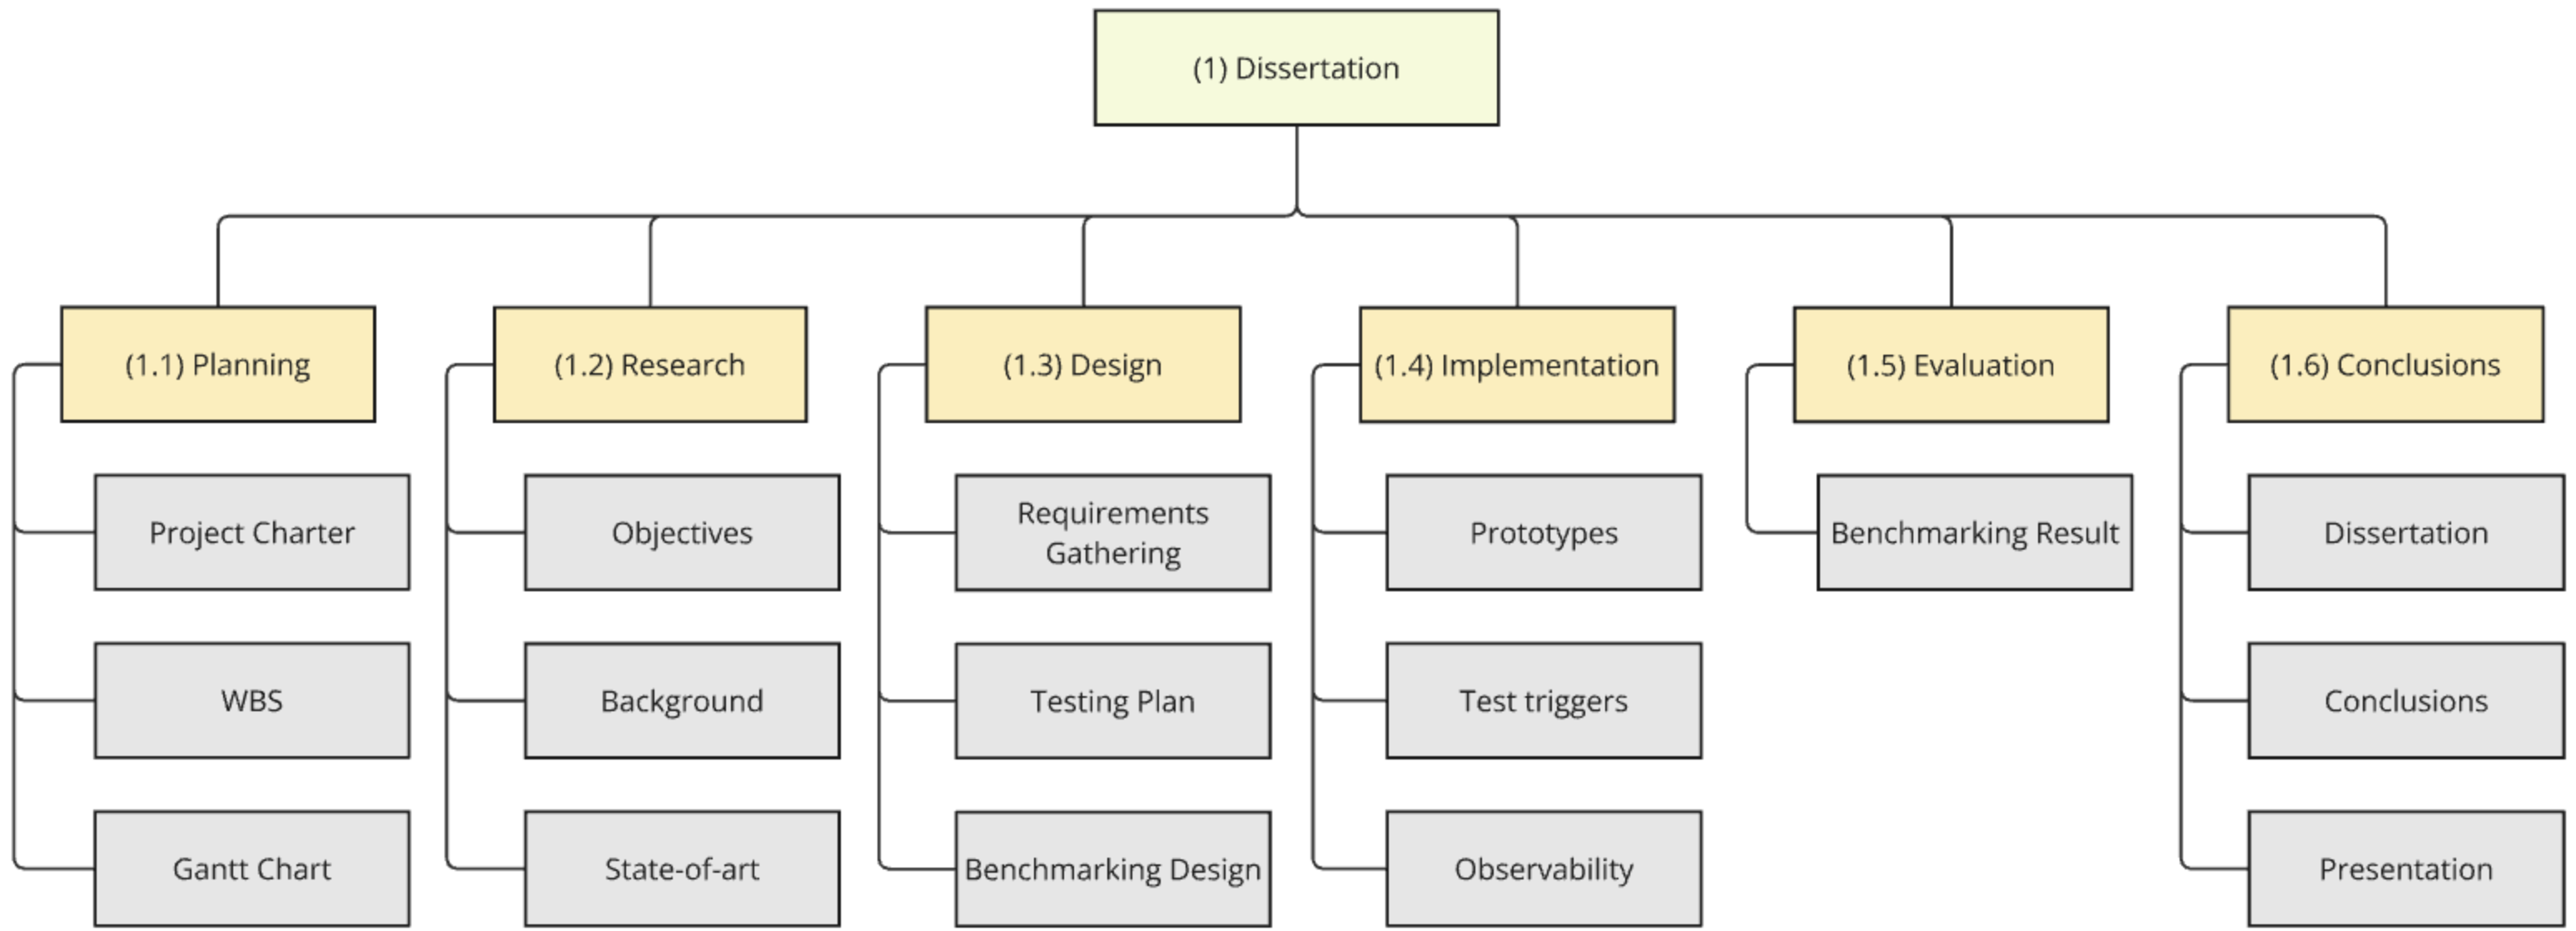
\includegraphics[width=\linewidth]{ch-planning/assets/wbs.png}
      \caption{The WBS of the project.}
      \label{fig:wbs}
\end{figure}

Due to the extension of the \gls{WBS} dictionary the table it is allocated on the appendix \nameref{AppendixA}. This table details each phase in order to be defined what are the goals and the acceptance criteria in a concise way. 

\section{Gantt Diagram}

This section provides details about the Gantt diagram, created using Microsoft Project. The timeline is illustrated in Figure \ref{fig:gantt_timeline}, where only the main phases, milestones, and the periodic schedule of control and feedback meetings are shown for simplicity. Additionally, the tasks covering the development of competencies are highlighted. Detailed information is provided below, offering an overview that demonstrates how the project’s organization aligns with the \gls{WBS}. For more in-depth details, refer to \nameref{AppendixA} for a representation of all tasks related.

\begin{figure}
      \centering
      \frame{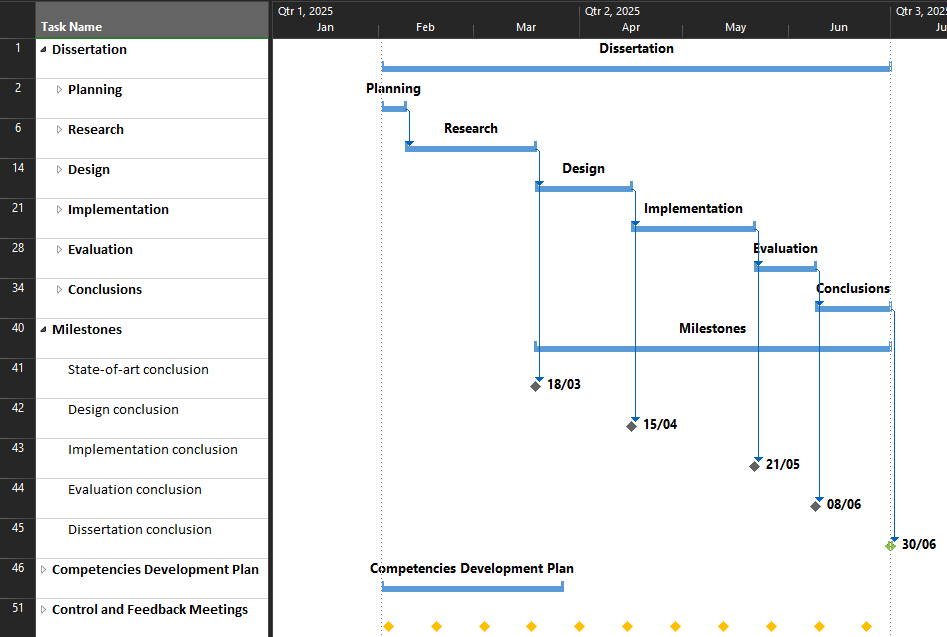
\includegraphics[width=\linewidth]{ch-planning/assets/gantt_timeline.png}}
      \caption{Gantt timeline of the project}
      \label{fig:gantt_timeline}
\end{figure}


\subsection{Project Management and Scheduling}

The project’s start date was set for 02/02/2025, following the first semester exams, with the end date aligned to the predefined project formalization deadline of 30/06/2025, as illustrated in Figure \ref{fig:gantt_timeline}. The scheduling strategy utilizes an automatic mode that calculates dates based on task durations and their interdependencies. This approach assumes a calendar with no restrictions on working days, treating all days, including weekends, as working days to facilitate continuous progress.

\paragraph{Estimation Rationale} Task durations were estimated by evaluating the complexity and importance of each project phase like illustrated by the column \textit{"Duration"} in Figure \ref{fig:gantt_monitoring}. The background and state of the art have a considerable slice, given their foundational role in the research. These stages demand research and analysis, making them time-consuming. Following this, the design phase received significant attention, as it involves defining system requirements and developing a detailed testing plan, which are important steps for the implementation.

The implementation phase was planned taking in considerations the necessity of prototyping, testing, and possible adjustments, making it the most time-consuming task. The evaluation phase, particularly benchmarking, was allocated less time compared to implementation, but enough time for a thorough analysis and interpretation of results. Finally, the conclusion phase was planned with a related similarly time to the state of the art to synthesize findings, document outcomes, and finalize the dissertation. Given the dependency between phases, this project is difficult to parallelize. The implementation phase relies heavily on the preceding design phase, and the evaluation phase depends on a functional implementation. 

\paragraph{Resource Allocation} A resource column was included in the project plan to track resource allocation, focusing on the student and advisor as the primary stakeholders as illustrated in Figure \ref{fig:gantt_timeline}. The advisor’s role is focused on controlling and monitoring tasks, providing feedback and guidance throughout the project.

\paragraph{Cost Management} The cost component was excluded from the project plan, as it is not applicable to this type of academic project.

\subsection{Monitoring and Controlling Procedures}

The strategy defined to have control over the progress of each task was to mark its progress by an estimated percentage of completion. This strategy ensures that the progress of the task is clearly visible and measurable, giving both the student and the advisor a view of progress, like it is possible to observe the \textit{“\% Completed”} column on the Figure \ref{fig:gantt_monitoring}.

To improve this process, specific tasks dedicated to monitoring and control have been incorporated, such as \textit{“Validation and Refinement with the Advisor”}, like illustrated in Figure \ref{fig:gantt_monitoring}. These tasks have two main objectives, firstly, to make the student responsible for presenting the partial document ready to be assessed. Secondly, to ensure that the advisor is warned in advance of the need for closer and more active feedback on these pre-defined days. Feedback can be given asynchronously via messages or synchronously during scheduled meetings. After the feedback time is up, the goal is to be able to present a refined partial document, referred to as the \textit{“Document version X”} task, also possible to observe in Figure \ref{fig:gantt_monitoring}.

\begin{figure}
      \centering
      \frame{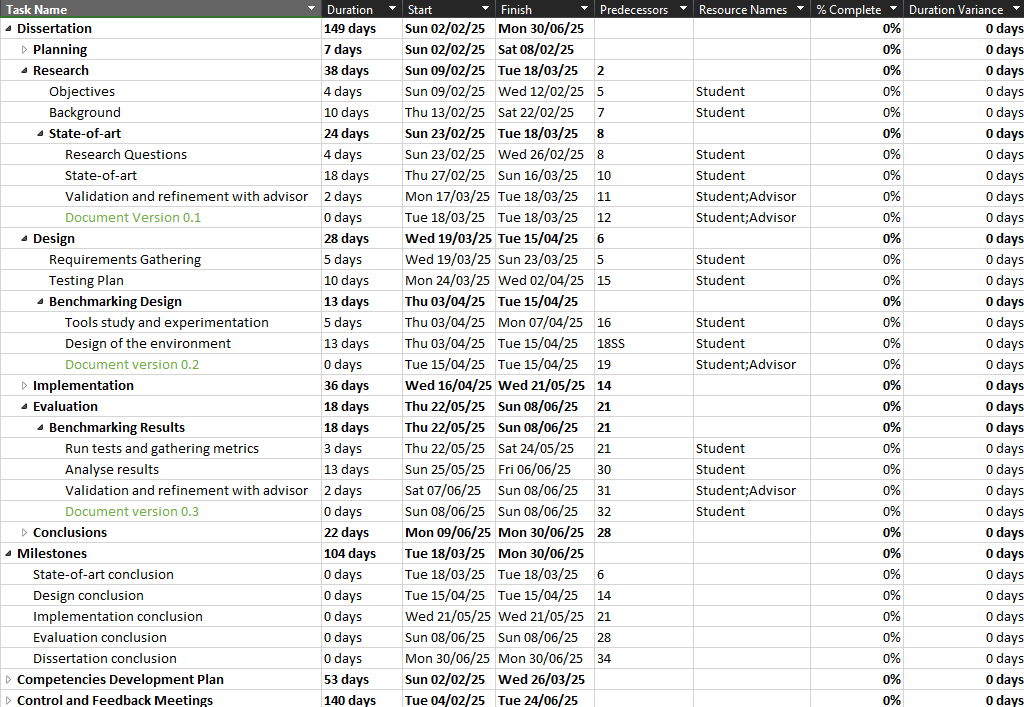
\includegraphics[width=\linewidth]{ch-planning/assets/gantt_monitoring.png}}
      \caption{Monitoring and control procedures displayed on the Gantt chart.}
      \label{fig:gantt_monitoring}
\end{figure}

Additionally, milestones have been defined to mark the completion of each significant project phase. These milestones serve as checkpoints to ensure progress is on track and can be observed in Figure \ref{fig:gantt_monitoring} under the main task \textit{“Milestones”}.

To manage potential delays, a baseline has been established. This baseline records the initial schedule, allowing deviations to be tracked throughout the project. This mechanism provides an overview of delays and their impact on the schedule. The column \textit{"Duration Variance”} column in Figure \ref{fig:gantt_monitoring} illustrates this feature, allowing a visualization of changes between planned and actual progress.

\subsection{Meeting Sessions}

To ensure consistent communication and effective progress monitoring with the advisor, a series of biweekly meetings has been scheduled on Wednesdays, with each session expected to last between 30 minutes and 1 hour. While the schedule includes a predefined list of sessions, it remains flexible, allowing adjustments to the frequency of meetings as the project evolves. For instance, the number of meetings may increase during the final stages of the project, at which point the Gantt chart should be updated accordingly.

\begin{figure}
      \centering
      \frame{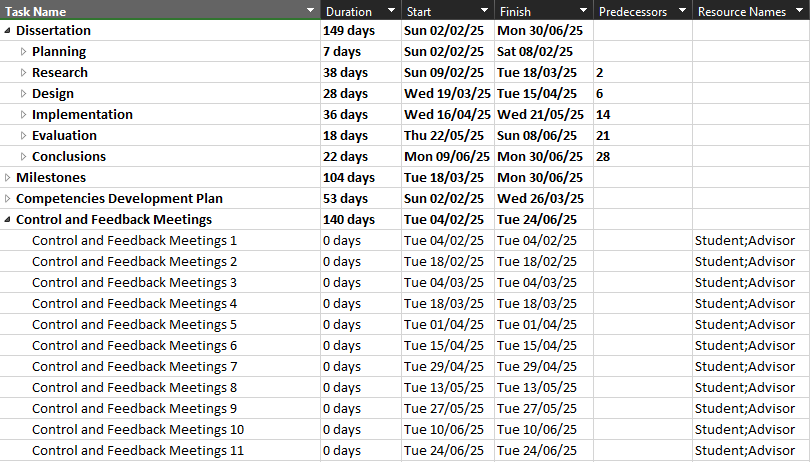
\includegraphics[width=\linewidth]{ch-planning/assets/gantt_meetings.png}}
      \caption{Meeting sessions represented on the Gantt chart.}
      \label{fig:gantt_meetings}
\end{figure}

The meeting schedule is illustrated in Figure \ref{fig:gantt_meetings}, which includes eleven recurring tasks organized under the main task \textit{“Meeting Sessions”}. These meetings are planned to take place online.

\subsection{Competencies Development Plan}

To address the competencies identified during the diagnosis of critical skills required for the completion of the dissertation, a dedicated section titled \textit{"Competencies Development Plan”} has been incorporated into the project plan, as illustrated in Figure \ref{fig:gantt_competency}. This section outlines targeted tasks designed to address these areas for improvement.

\begin{figure}
      \centering
      \frame{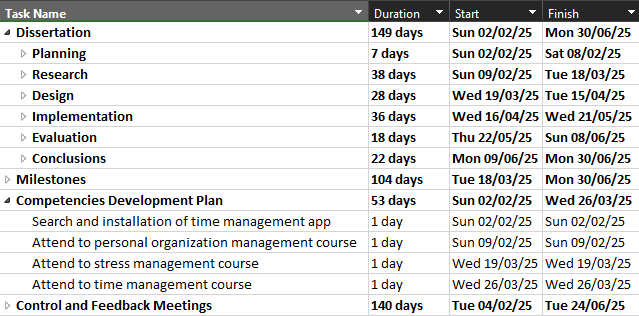
\includegraphics[width=\linewidth,scale=0.5]{ch-planning/assets/gantt_skills.png}}
      \caption{Competencies development plan represented on the Gantt chart.}
      \label{fig:gantt_competency}
\end{figure}

For stress management and resilience, the plan includes attending a "Stress Management" course\footnote{Managing Stress Course: \url{https://www.linkedin.com/learning/managing-stress-2019/} (accessed 4 January 2025)}. To enhance self-discipline and time management, the initial task involves identifying and installing at least one productivity application, such as tools that restrict smartphone usage during certain periods, for example. Additionally, time management competence is further explored by taking the "Time Management Fundamentals" course\footnote{Time Management Fundamentals Course: \url{https://www.linkedin.com/learning/time-management-fundamentals-14548057/the-power-of-managing-your-time/} (accessed 4 January 2025)}.

Communication, another key area of focus, will be developed by attending to the "Communicating with Confidence" course\footnote{Communicating with Confidence Course: \url{https://www.linkedin.com/learning/como-se-comunicar-com-confianca/} (accessed 4 January 2025)}.

\section{Risk Management}

Effective risk management seeks to transform potential uncertainties into more predictable and controlled outcomes. To achieve this, the most significant risks identified are described next

\subsection{Risk 1: Bugs in Third-Party Libraries}

\textbf{Description:} There is a potential risk of encountering bugs in third-party libraries, which could compromise the viability of implementation and testing of the prototypes. Since the project relies on external libraries to implement fault-tolerant strategies, the stability and reliability of these libraries are important.

\textbf{Cause:} The cause of this risk is the need of trust on external software components.

\textbf{Effect on the Project:} Errors in the libraries can compromise the viability of the prototype's development and also the integrity of the results.

\textbf{Risk Owner:} Student.

\textbf{Probability.} 2. \textbf{Impact:} 4. \textbf{PI Score.} 8.

\textbf{Risk Response Strategy:} To mitigate this risk, alternative libraries will be identified for each strategy and language in advance. At least two or three libraries will be shortlisted and prioritized. If the primary library encounters significant bugs or issues, the next library on the list will be utilized.

\textbf{Expected Result Without Action:} If no action is taken, delays in prototypes development will occur.

\textbf{Risk Response Type:} Mitigation.

\textbf{Response Description:} A proactive approach will be taken to evaluate multiple libraries during the research phase.


\subsection{Risk 2: Integration Challenges Between Components}

\textbf{Description:} Integration issues could arise when combining multiple components, such as third-party libraries, testing frameworks, and custom implementations.

\textbf{Cause:} Differences in interfaces, versions, or dependencies among components used in the project.

\textbf{Effect on the Project:} These challenges could delay testing and result in compatibility issues that reduce productivity.

\textbf{Risk Owner:} Student.

\textbf{Probability.} 2. \textbf{Impact:} 4. \textbf{PI Score.} 8.

\textbf{Risk Response Strategy:} To mitigate this risk, dependencies and versions will be carefully managed using dependency management tools. Component integration will also be tested incrementally to identify issues early.

\textbf{Expected Result Without Action:} Significant delays during the integration of components on the implementation phase.

\textbf{Risk Response Type:} Mitigation.

\textbf{Response Description:} Incremental integration practices will ensure smoother component interaction.